%!TEX root = ../report.tex

\begin{document}
    \chapter{Solution}
        Due to causes unrelated to this project, the available data was just one CityGML model and its corresponding point cloud.
        Therefore, a solution was designed based on this data and its characteristics.

        Later, in the middle phase of the project, another point cloud was available but its corresponding CityGML model was not.
        However, instead of a CityGML model, a 3D model of the site was available in Polygon File Format (ply).
        Because of the different information contained in the PLY file a different preprocessing was needed.

        Although (deep) learning methods are very attractive due to their boom in recent years,
        they are unthinkable to solve our problem. The main reason for this is the data needed to train such an approach.

        Goebbels et al. \cite{Goebbels_2018_linebased, Goebbels_2018_alinear} successfully propose the use of Mixed Integer Linear Programming to register
        a point cloud with a CityGML model, based on lines and points.
        Mixed Interger Linear Programming has been used to solve other registration problems
        like the registration between two point clouds \cite{Sakakubara_2007_automatic},
        registration between 3D shapes \cite{Windheuser_2011_largescale},
        and 2D registration \cite{Bazin_2013_abranchandbound}.

        Therefore, the solution proposed is to detect the walls in the point cloud and the 3D model by projecting both onto the xy-plane,  
        and then use the angles of the corners of the walls (where the walls intersect)
        in a Mixed Integer Linear Program to find correspondences and a transformation that aligns the point cloud with the 3D Model at the same time.
        The exact details are given in the next section.

        From now on, the point cloud could be referred to as the source, and the 3D model as the target.
     
%-------------------------------------------------------------------------------
%	Proposed algorithm
%-------------------------------------------------------------------------------
    \section{Proposed algorithm}
        The main steps of the proposed algorithm are listed as follows:
        \begin{enumerate}
            \itemsep 0em 
            \item Projection of the point cloud onto the xy-plane.
            \item Projection of the 3D model onto the xy-plane.
            \item Detection of line segments.
            \item Detection of line intersections and their angles.
            \item Identification of possible correspondences between angles detected.
            \item Alignment of both projections onto the xy-plane.
            \item Alignment on the z-axis.
        \end{enumerate}

    %-------------------------------------------------------------------------------
    %	Projection of the point cloud onto the xy-plane
    %-------------------------------------------------------------------------------
        \subsection{Projection of the point cloud onto the xy-plane}
        \label{sub:Projection of the point cloud onto the xy-plane}
            To simplify the registration task, this is transported from the 3D space to the 2D space.
            As we can see in \autoref{fig:initial_front_model} and \autoref{fig:initial_back_model}, 
            the z-axis of the source and the target is already correctly aligned.
            Which allows for a direct projection of the source onto the xy-plane to detect walls.

            \begin{figure}[H]
                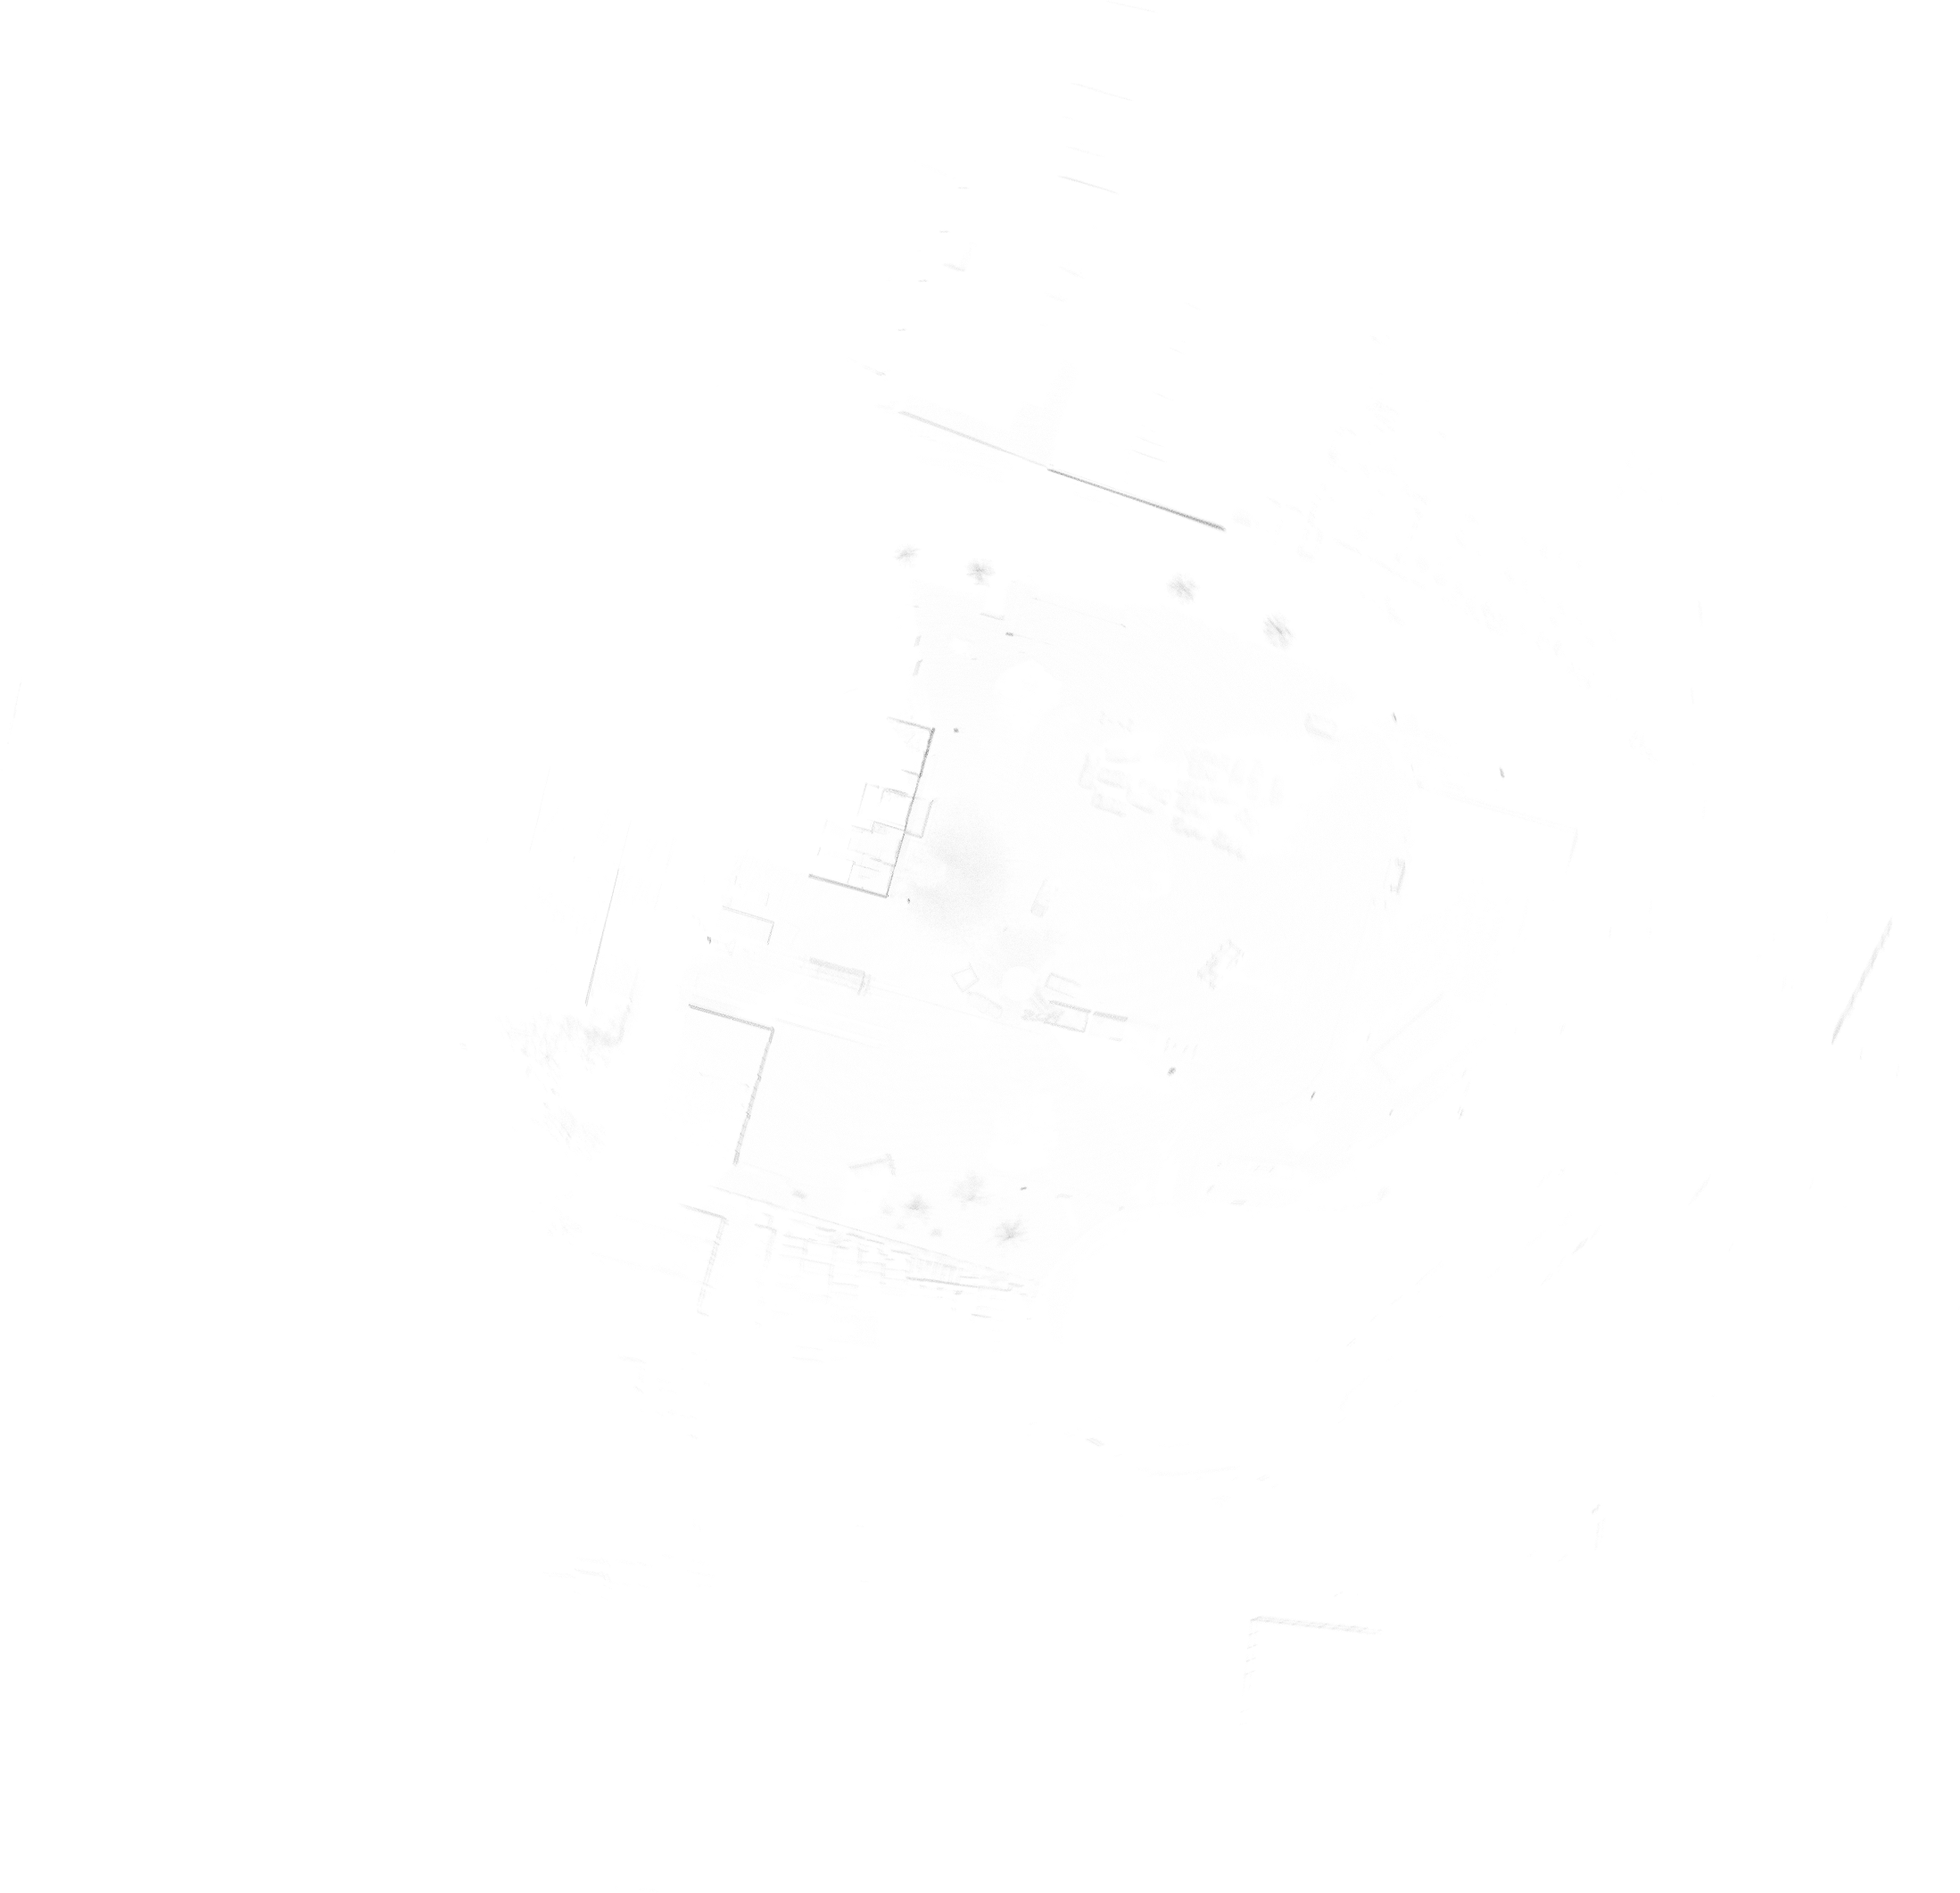
\includegraphics[width=\textwidth]{images/solution_images/source_image_inverted.png}
                \caption{Projection of the source onto the xy-palne.}
                \label{fig:source_image}
            \end{figure}

            To project the source onto the xy-plane, one can create an empty image with enough size for the source and the target to fit.
            Then, one can sum the number of points in the source with the same x- and y-coordinates and write the result in the corresponding pixel in the image.
            In this way, we can obtain a view of the source from bellow where line segments depict walls.
            \autoref{fig:source_image} shows the image obtained after the projection of the source.
            

    %-------------------------------------------------------------------------------
    %	Projection the 3D model onto the xy-plane
    %-------------------------------------------------------------------------------
        \subsection{Projection the 3D model onto the xy-plane}
            \begin{figure}[H]
                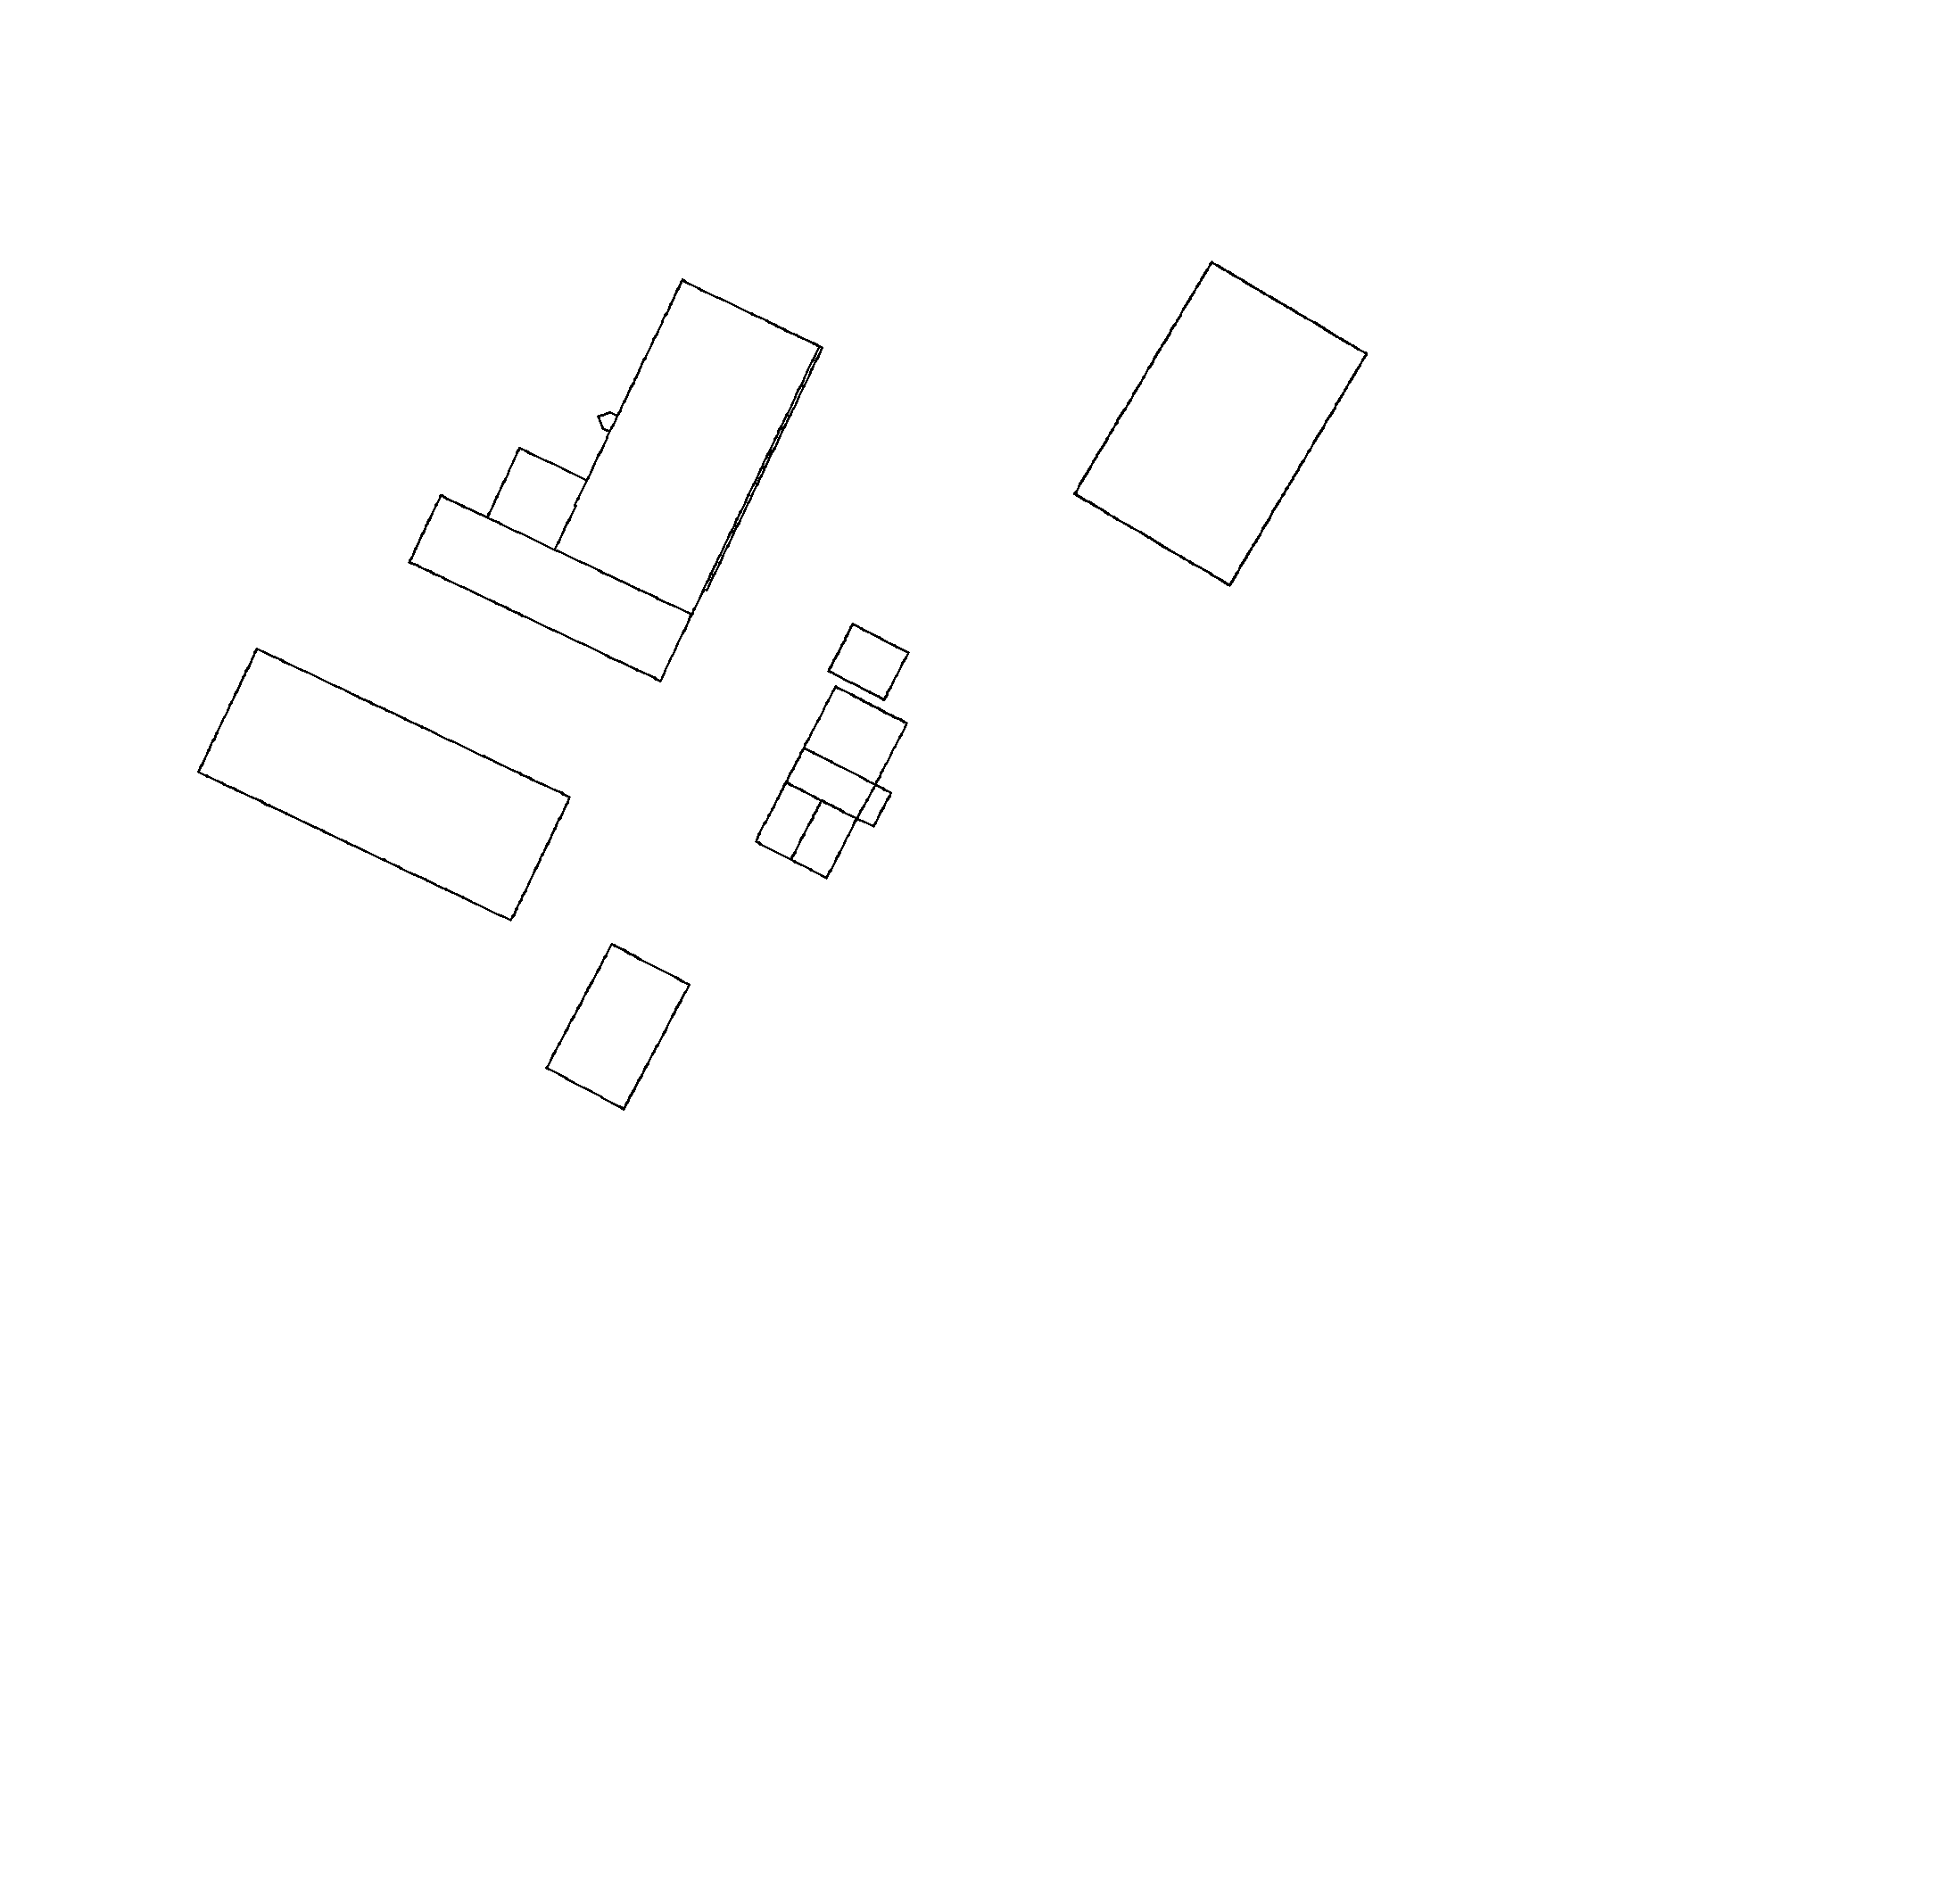
\includegraphics[width=\textwidth]{images/solution_images/target_image_inverted.png}
                \caption{Projection of the target onto the xy-palne.}
                \label{fig:target_image}
            \end{figure}

            The difference between using CityGML Models and the PLY models relies on their projection onto the xy-plane.
            From the PLY model, a point cloud is sampled and projected onto the xy-plane as described in \autoref{sub:Projection of the point cloud onto the xy-plane}.

            Fortunately, the CityGML model already provides a terrain intersection.
            From this terrain intersection, only the x- and y-coordinates are used to make the projection.
            In an empty image, line segments are drawn from point to point so that a footprint is obtained.

            \autoref{fig:target_image} shows the image obtained after this process.

            
    %-------------------------------------------------------------------------------
    %	Detection of line segments
    %-------------------------------------------------------------------------------
        \subsection{Detection of line segments}
            \begin{figure}[H]
                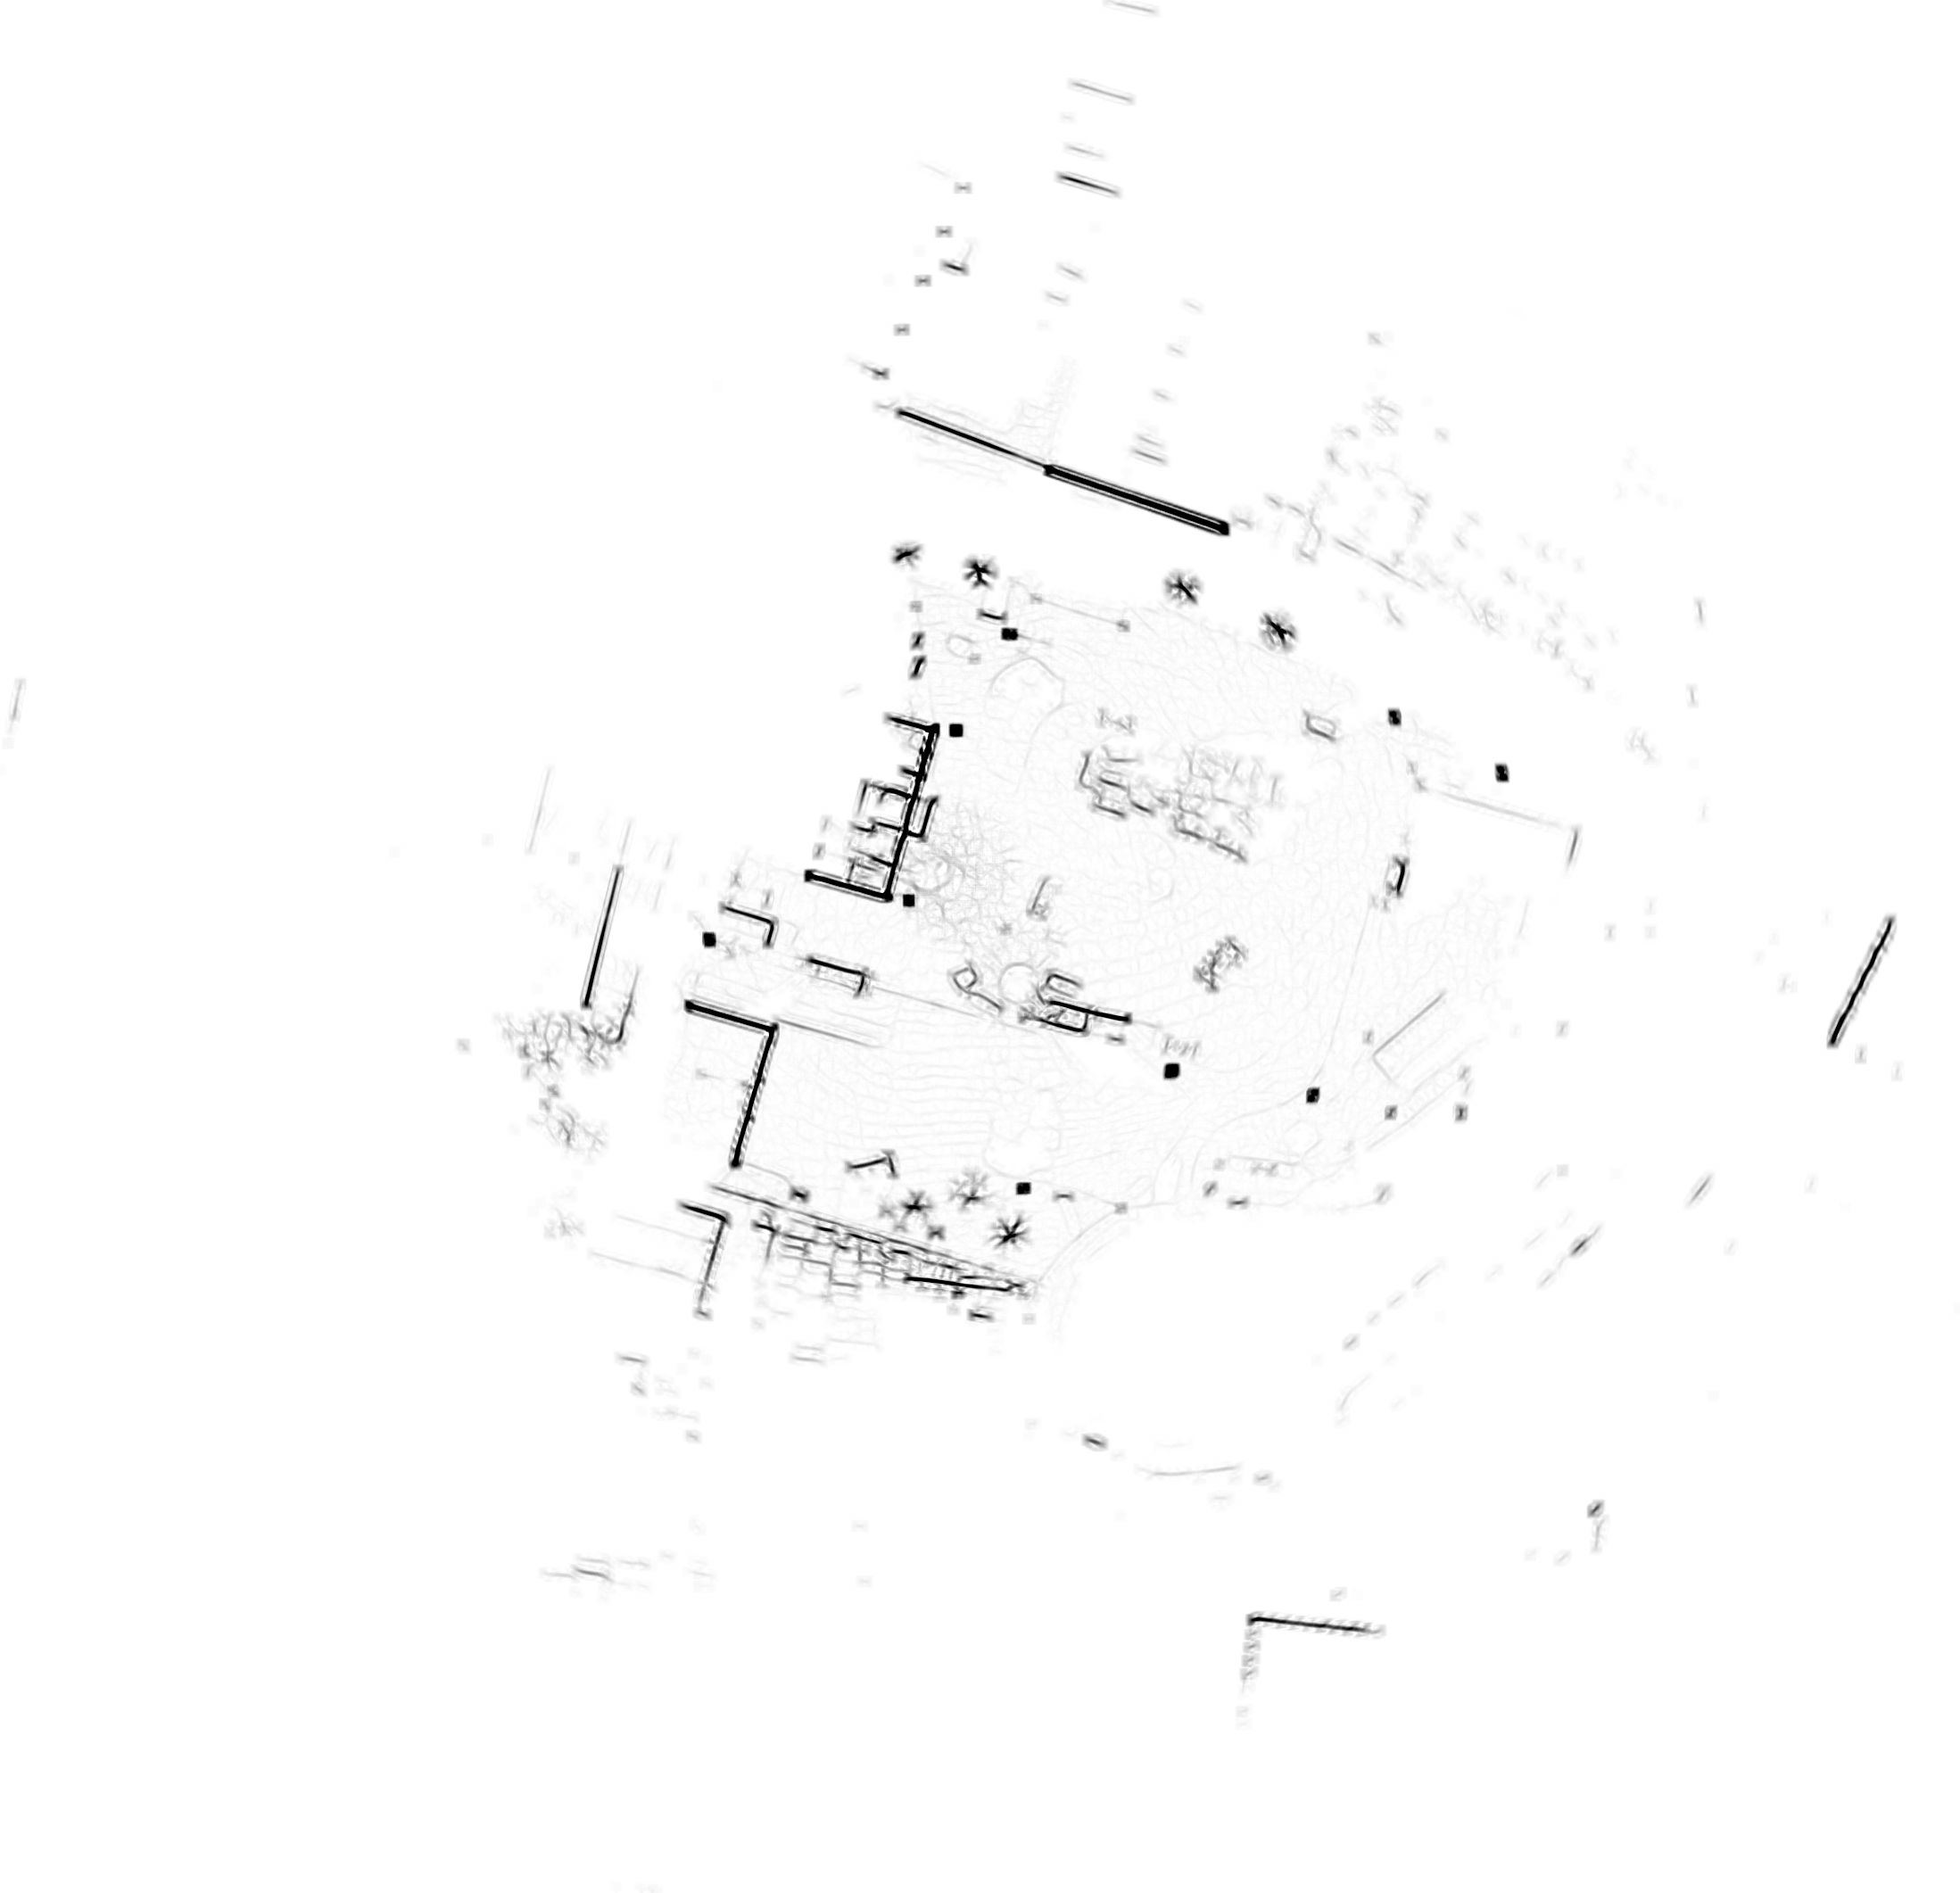
\includegraphics[width=\textwidth]{images/solution_images/filter_inverted.png}
                \caption{Source image after filter.}
                \label{fig:source_image_filter}
            \end{figure}
        
            The projections of the source and the target are now 2D images. 
            The source image could be noisy, but the target is clear and the line segments that represent the walls are very well defined.
            Therefore, to deal with the noise and remark the line segments of the source image an implementation of the technique proposed 
            by Chaudhuri et al. \cite{Chaudhuri_1989_detection}, to detect blood vessels in retinal images, together with a binary threshold is used. 
            The implementation of \cite{Chaudhuri_1989_detection} used is the one provided by DIPlib \cite{DIPlib_online}.
            \autoref{fig:source_image_filter} shows the result after the filter is applied to \autoref{fig:source_image}.

            Line segments in both images are detected using the probabilistic hough line transform of OpenCV \cite{opencv_library}.
            The number of line segments is reduced in four steps. 
            Firstly, short line segments are deleted, i.e. line segments with lengths lower than a given threshold.
            Secondly, line segment s with similar slopes are identified. 
            Then, from this set of line segments, subsets of line segments with close starting and ending points are created,
            and only the longest one of each set is preserved. The rest of the line segments are deleted.
            Thirdly, line segments with similar inclination angles are detected, and the same as in the second step is done.
            Finally, line segments with similar angles that are too close are merged by eliminating or extending one of the line segments.

    %-------------------------------------------------------------------------------
    %	Detection of line intersections and their angles
    %-------------------------------------------------------------------------------
        \subsection{Detection of line intersections and their angles}
            \begin{figure}[H]
                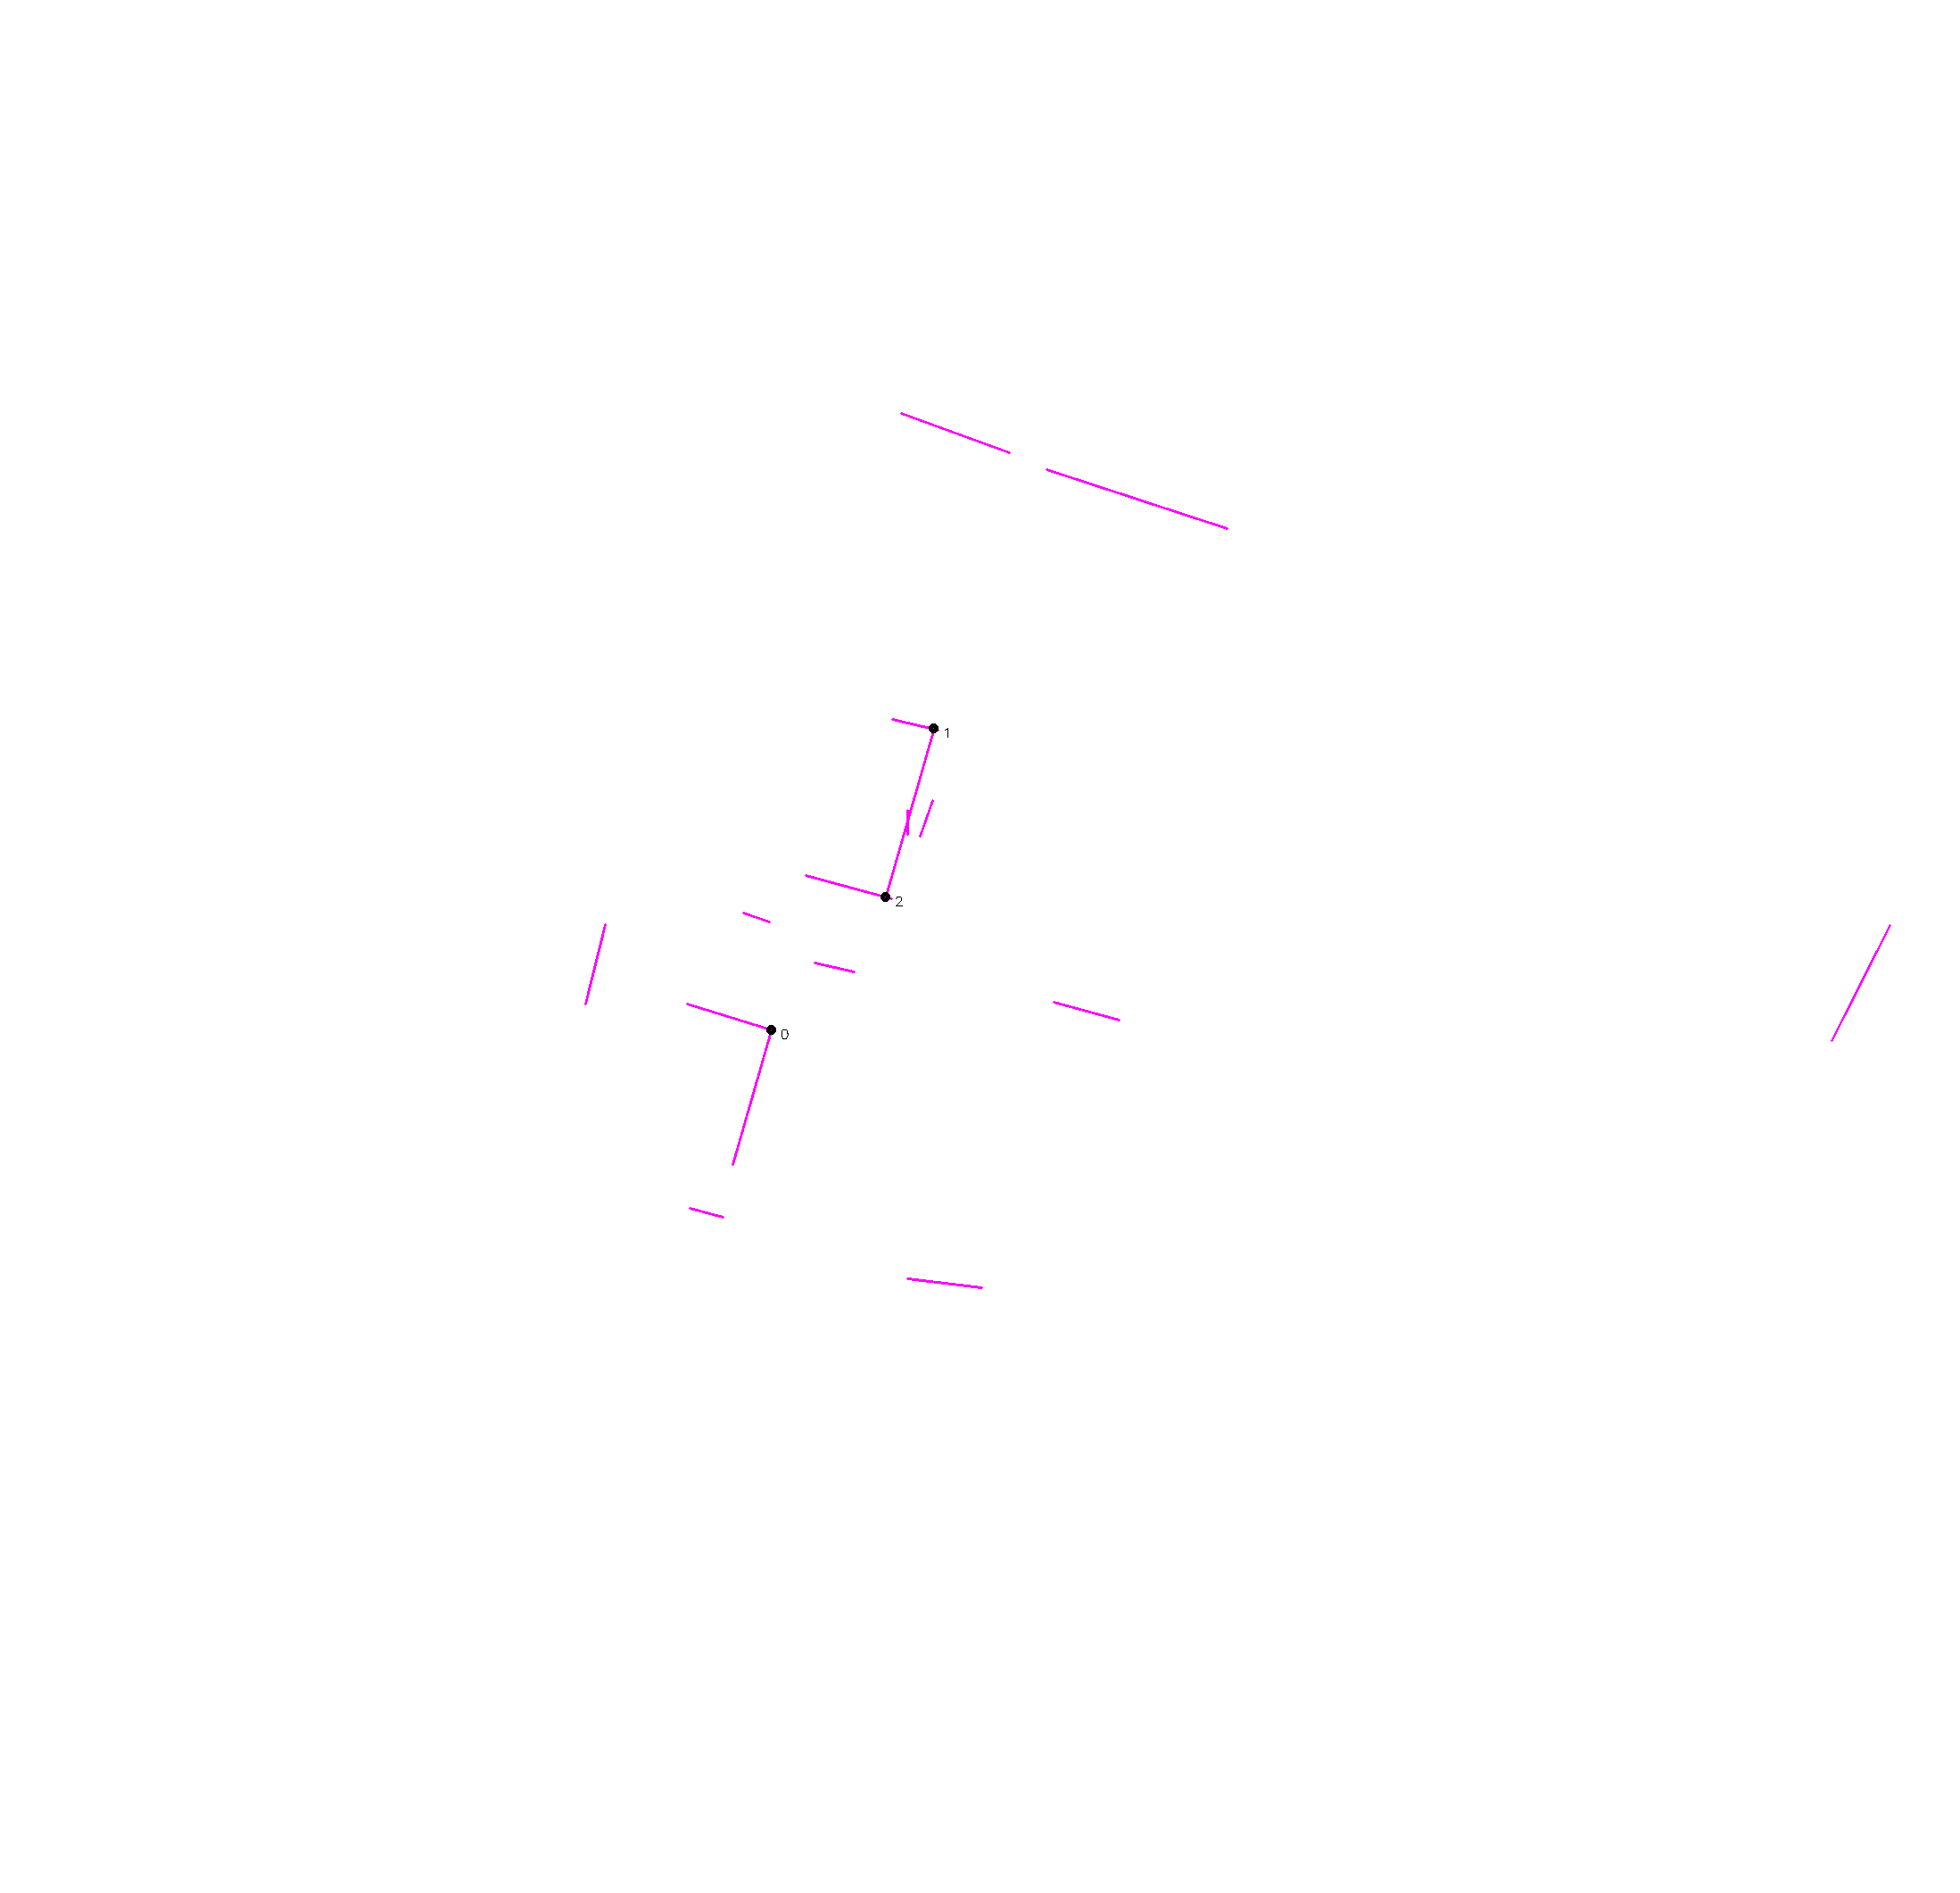
\includegraphics[width=\textwidth]{images/solution_images/source_intersections_inverted.png}
                \caption{Source lines and intersections.}
                \label{fig:source_intersections}
            \end{figure}

            \begin{figure}[H]
                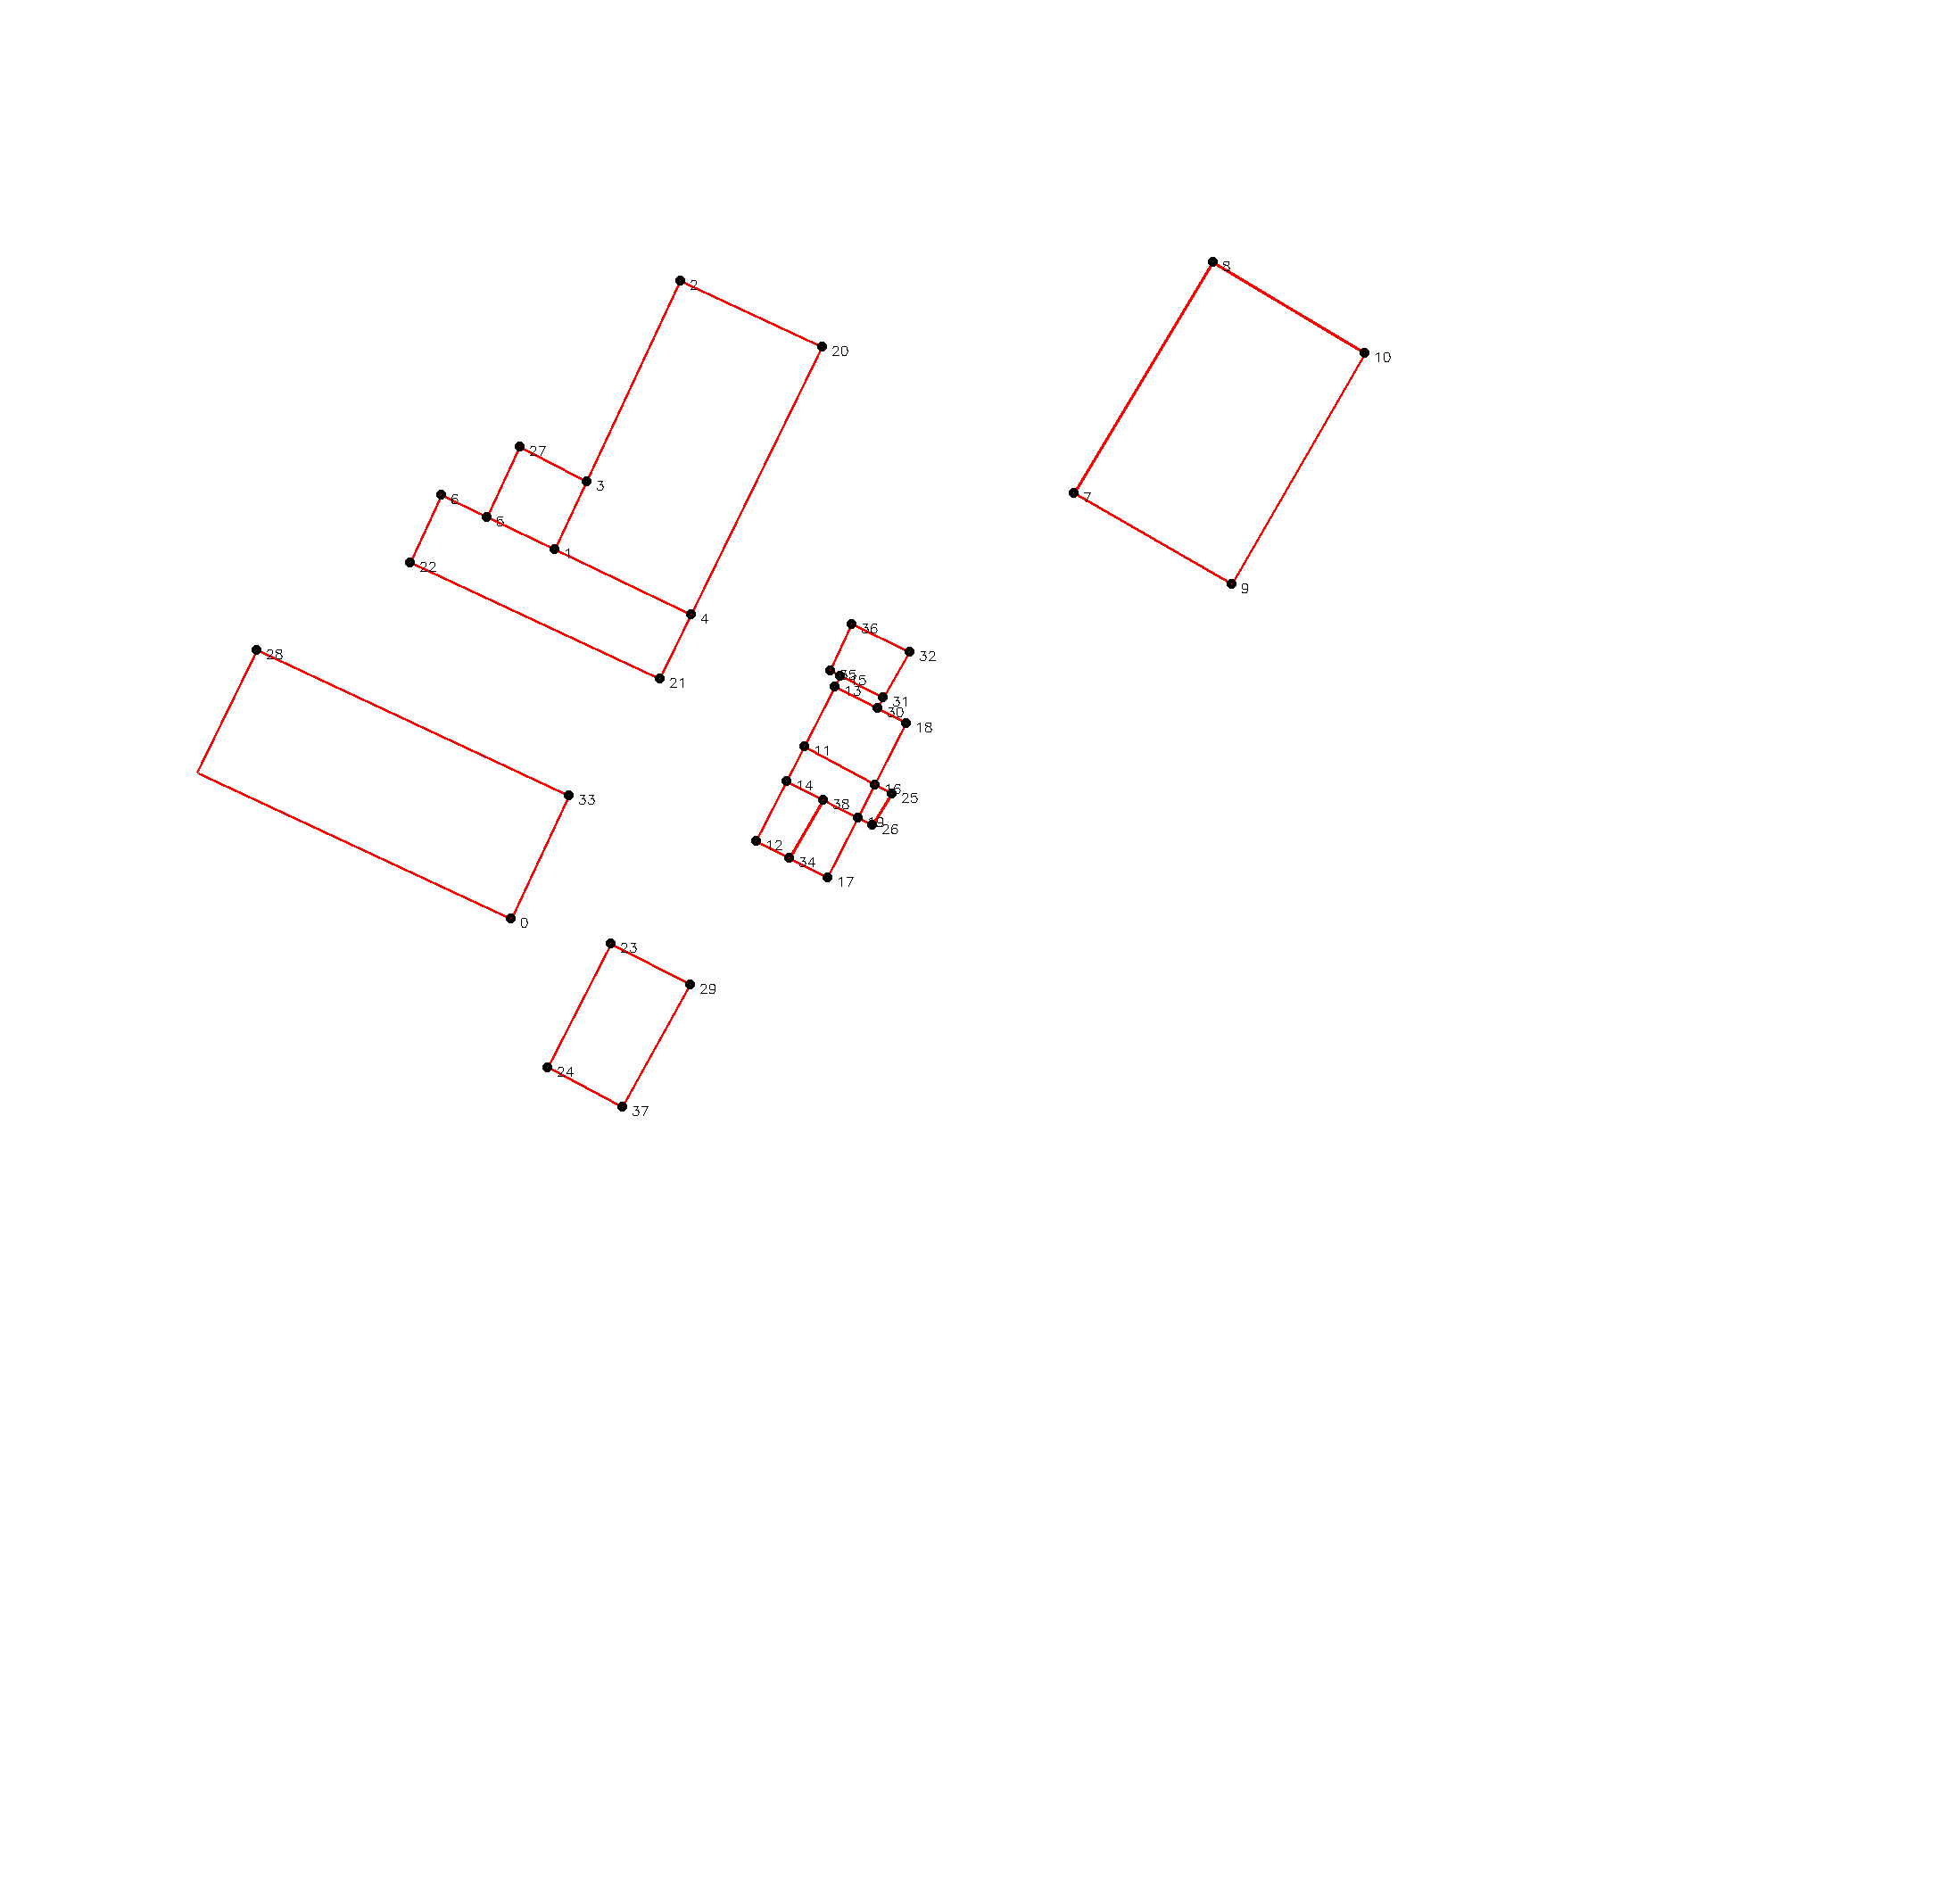
\includegraphics[width=\textwidth]{images/solution_images/target_intersections_inverted.png}
                \caption{Target lines and intersections.}
                \label{fig:target_intersections}
            \end{figure}

            The line segments are converted to their homogeneous representation, 
            and the intersections between them are calculated using the cross product as described in \cite{Hartley_2003_multiple_Book}.
            Only the intersections that are in the line segments are taken into account.
            Then, the angles of the intersections are computed.

            The intersections detected in the source image and the target image are now the set of points $P$ and $Q$, respectively, 
            as described in \autoref{section:Registration Problem in 2D}. 
            \autoref{fig:source_intersections} shows $P$ and \autoref{fig:target_intersections} shows $Q$.


    %-------------------------------------------------------------------------------
    %	Identification of possible correspondences between angles detected
    %-------------------------------------------------------------------------------
        \subsection{Identification of possible correspondences between angles detected}
            The angles of the intersections in the source image and the target image are compared,
            and if they are similar to each other, they represent a possible match.

            More formally, there is a matrix $C \in \mathbb{R}^{N \times M}$ that represents the possible correspondences.
            That means that $c_{ij} = 1$ if the angle $i$ in the source image is similar to the angle $j$ in the target image.
            Otherwise, $c_{ij} = 0$.

    %-------------------------------------------------------------------------------
    %	Alignment of both projections onto the xy-plane
    %-------------------------------------------------------------------------------
        \subsection{Alignment of both projections onto the xy-plane}
            \label{sub:Alignment of both projections onto the xy-plane}

            \begin{figure}[H]
                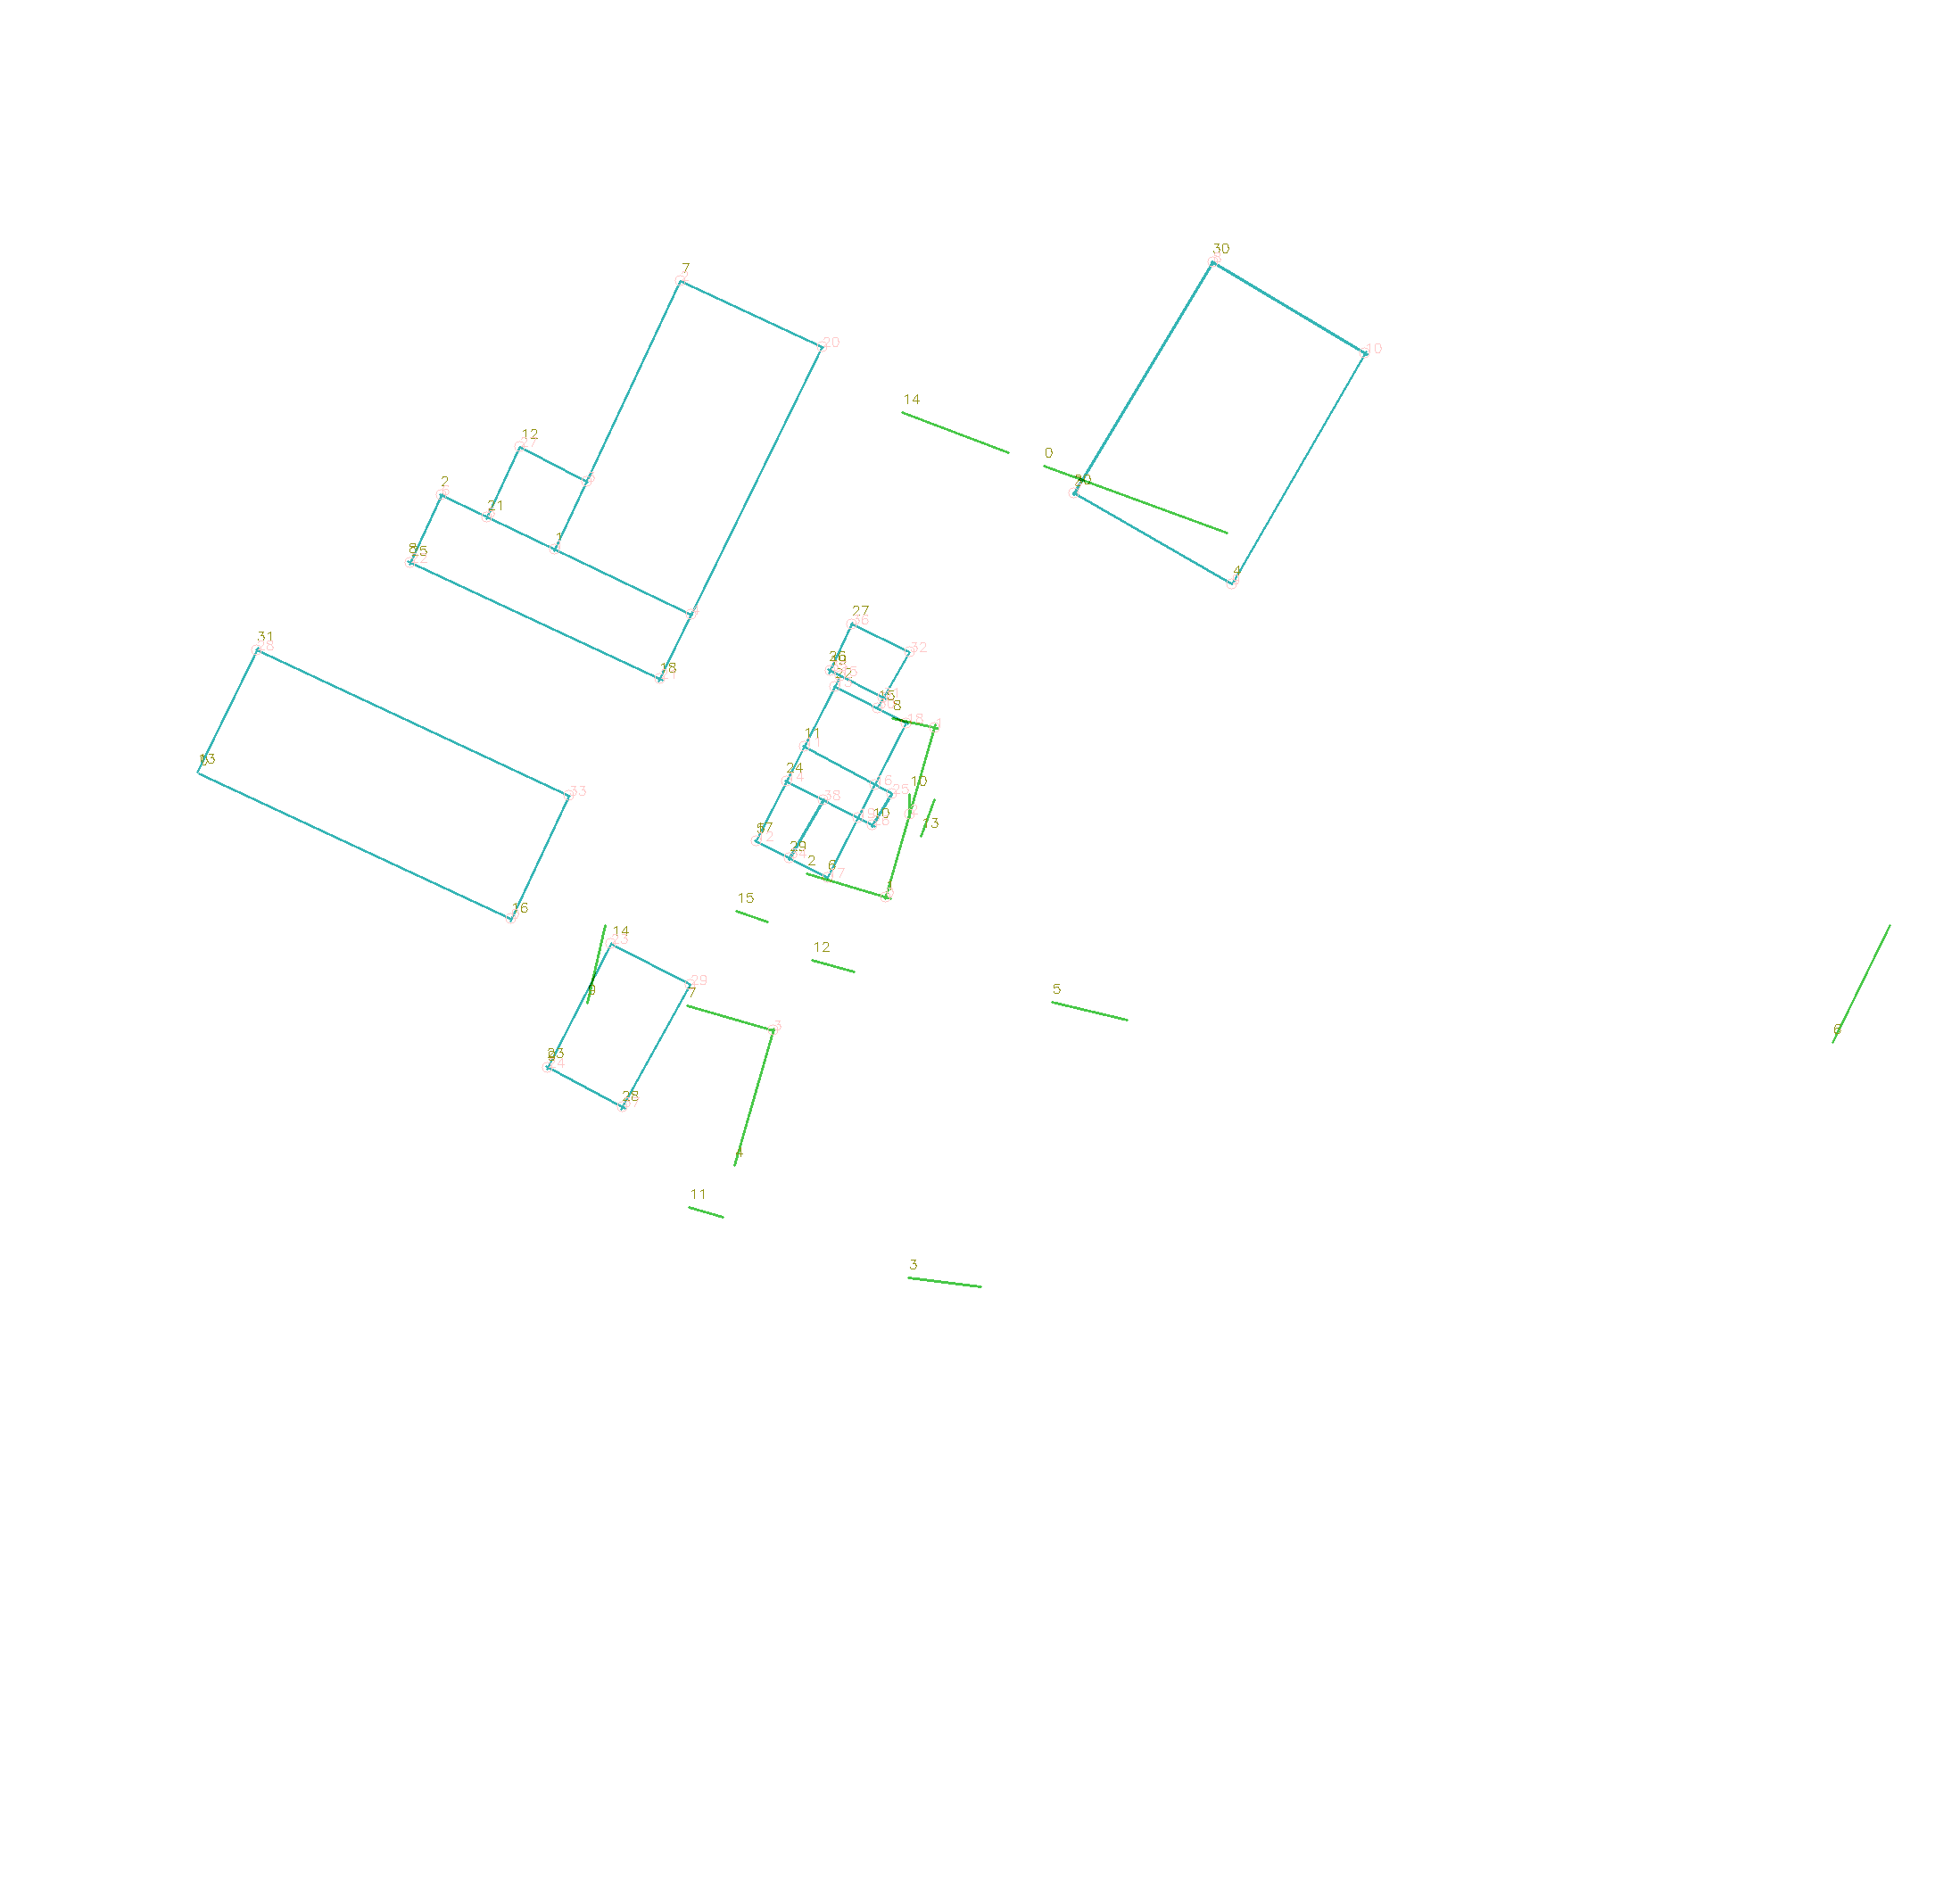
\includegraphics[width=\textwidth]{images/solution_images/2D_XY_initial_inverted.png}
                \caption{Initial position of the source image and the target image.}
                \label{fig:2D_initial}
            \end{figure}

            \begin{figure}[H]
                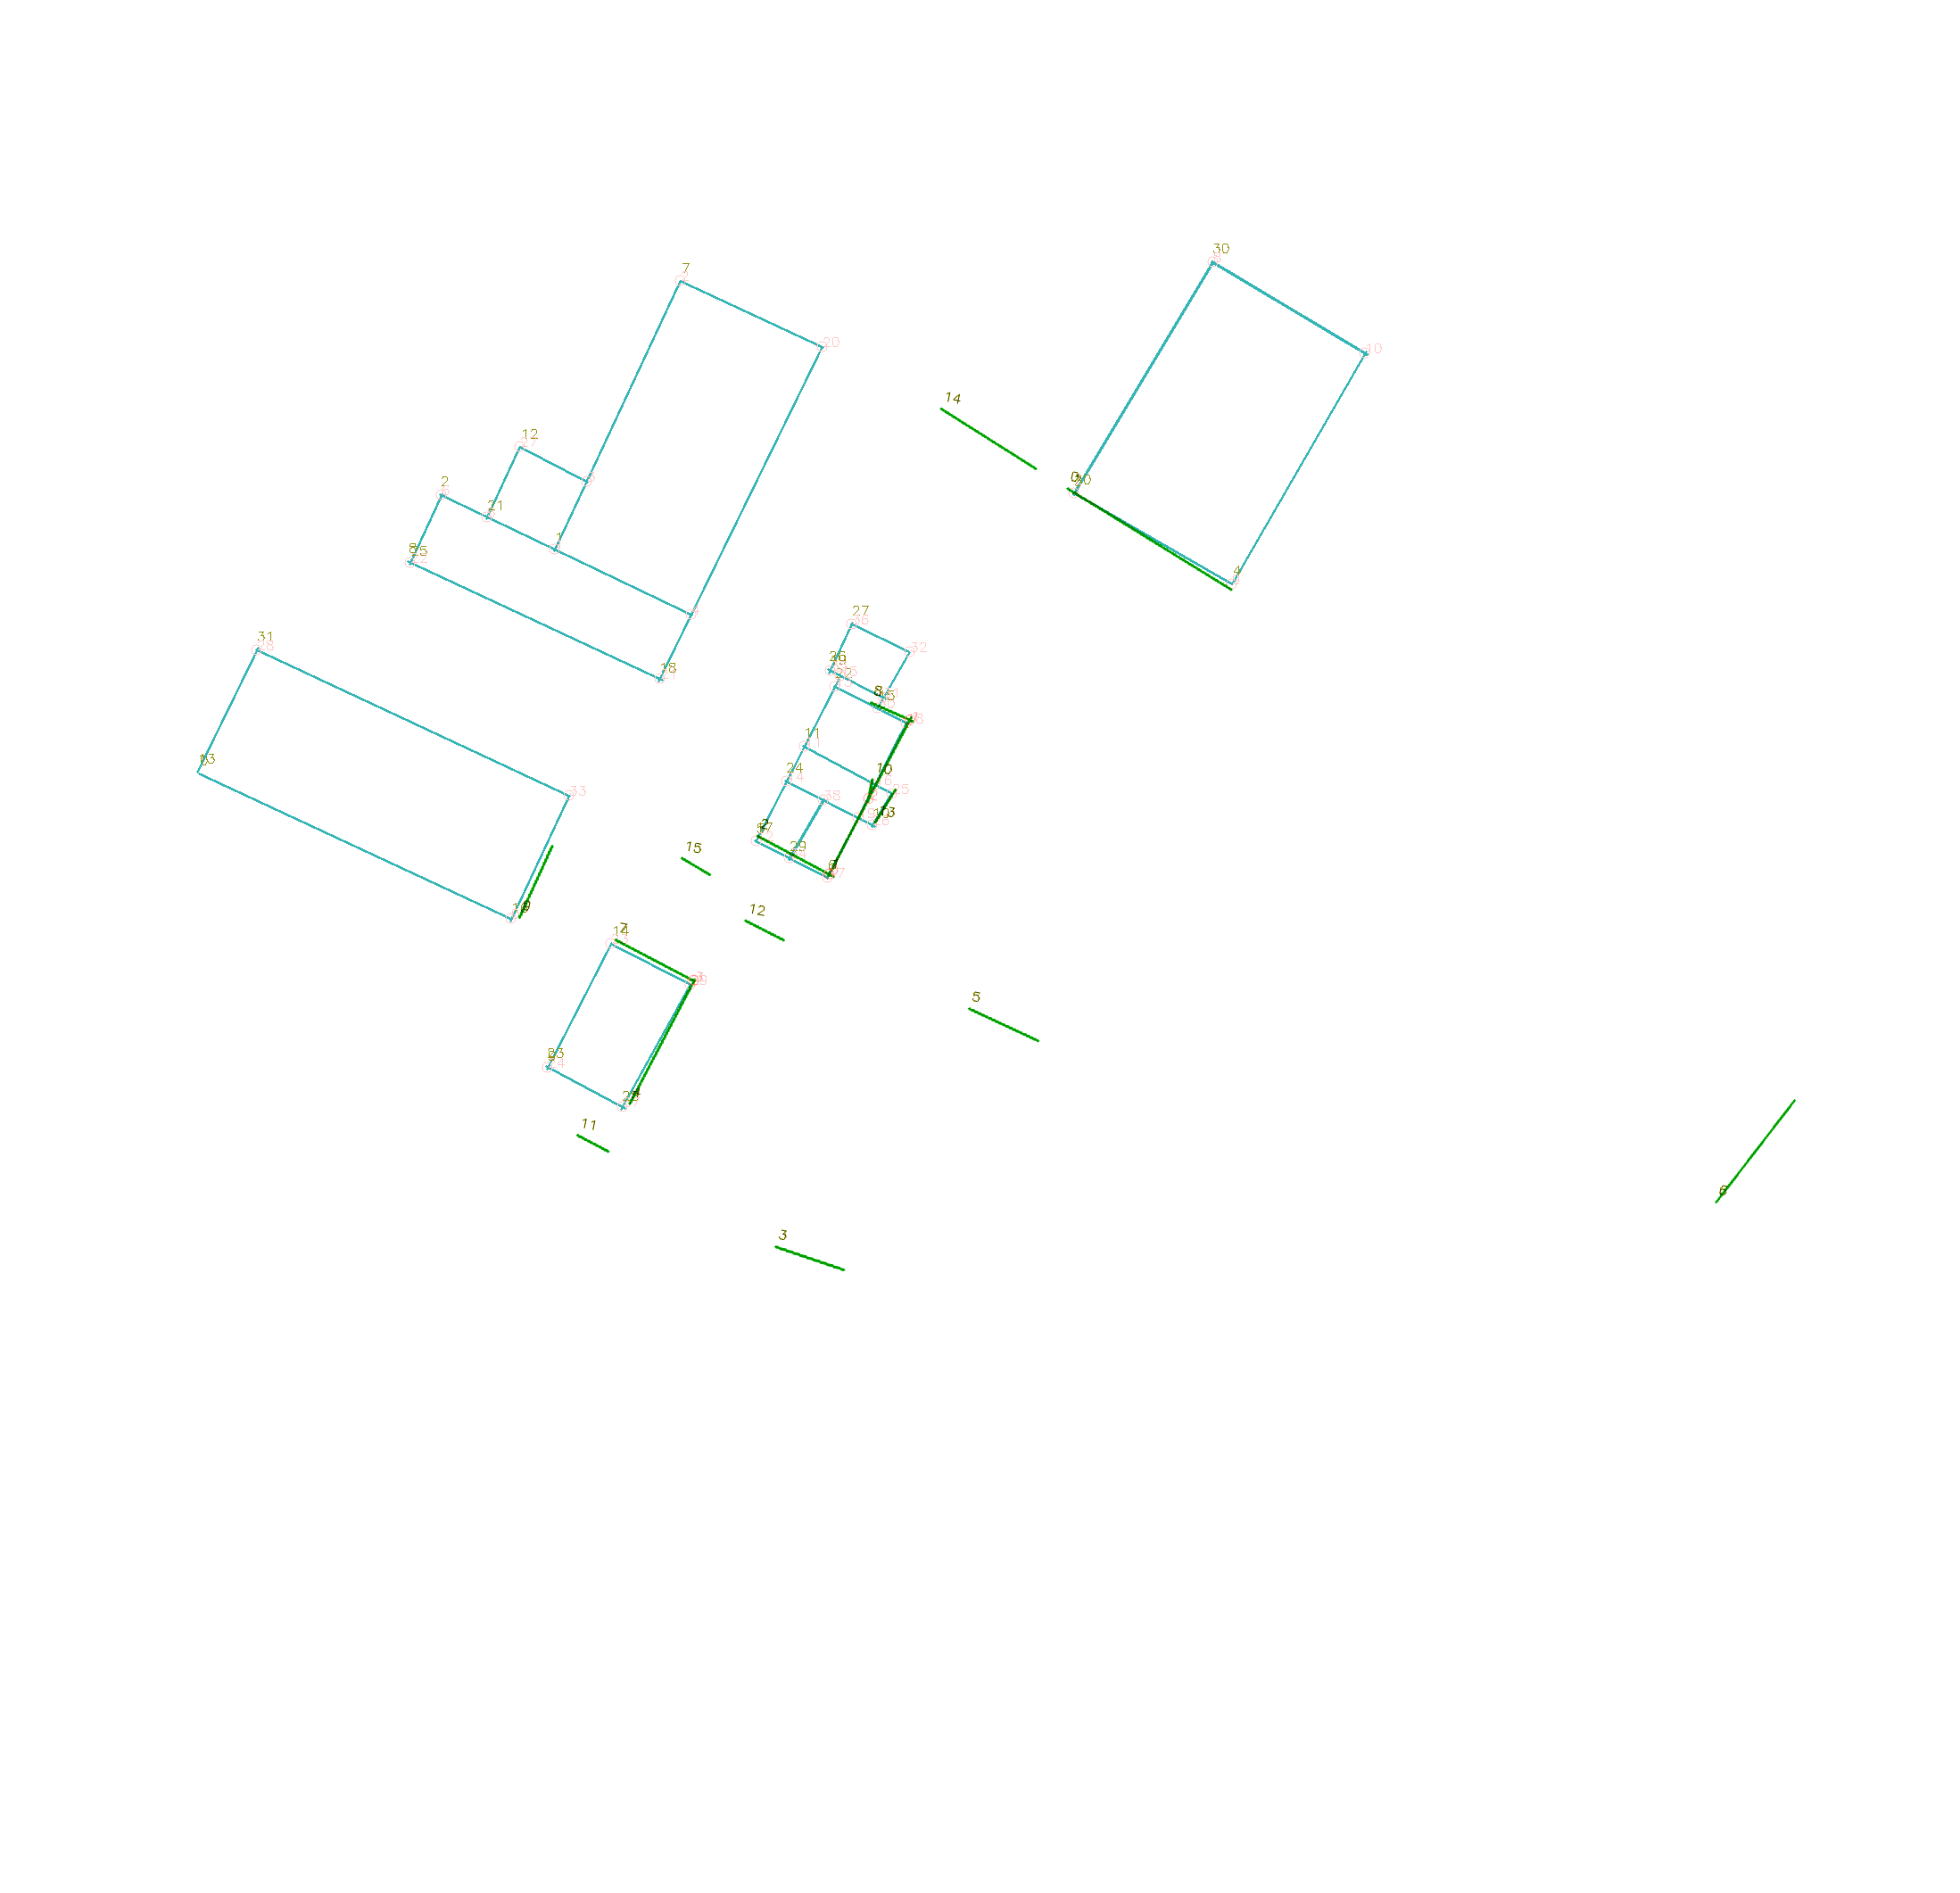
\includegraphics[width=\textwidth]{images/solution_images/2D_XY_alignment_inverted.png}
                \caption{Source image and target image aligned.}
                \label{fig:2D_aligned}
            \end{figure}

            The Mixed Integer Linear Program of \autoref{section:Registration Problem as Mixed Integer Linear Program} is solved with the intersections detected.
            The objective is changed to speed up the Mixed Integer Linear Program. The new objective is to maximize

            \begin{equation}
                \label{eq:objective_angles}
                \sum_{i}^{N} \sum_{j}^{M} x_{ij} m_{ij} 
            \end{equation}    

            subject to the constraints presented in \autoref{section:Registration Problem as Mixed Integer Linear Program}.
            This change in the objective adds additional information about the correspondences and significantly reduces the computation time.

            The Mixed Integer Linear Program is solved and the result is a transformation $T$ that aligns the source image with the target image,
            and a matrix $X$ that represents the correspondences between $P$ and $Q$.

            \autoref{fig:2D_initial} shows the initial position of the source image and the target image.
            \autoref{fig:2D_aligned} shows the result after the transformation of the source image with $T$.

            Because the source image and the target image are a projection onto the xy-plane of the source and the target, respectively,
            $T$ is used to align the source and the target on the x-axis and the y-axis by expanding it into the $SE(3)$.

    %-------------------------------------------------------------------------------
    %	Alignment on the z-axis
    %-------------------------------------------------------------------------------
        \subsection{Alignment on the z-axis}
            Sometimes a translation across the z-axis is needed to align the source and the target completely.
            The correspondences found in \autoref{sub:Alignment of both projections onto the xy-plane} 
            can be used to find the l

            If $x_{ij} = 1$ then the points $p_i$ and $q_j$ are used in the following way.
            The point $p_i$ is used to find the lowest point $p_i^l$ in the source with x- and y-coordinates similar to those of $p_i$.
            And the point $q_j$ is used to find the lowest point $q_j^l$ in the source with x- and y-coordinates similar to those of $q_j$.
            Then, the difference along the z-axis between $p_i^l$ and $q_i^l$ is computed.
            Finally, an average of all the differences computed is the translation $t_z$, which is then integrated into the transformation $T$.

%-------------------------------------------------------------------------------
%	Implementation details
%-------------------------------------------------------------------------------
    \section{Implementation details}
        - Python
        - libraries
        - 

\end{document}
